% CREATED BY MAGNUS GUSTAVER, 2020
\chapter{First Appendix}
\lipsum[1]


\subsection{random sample}

%disitrbution error historgram
\begin{figure}[ht]
    \centering
    \begin{subfigure}[t]{0.5\textwidth}
        \centering
        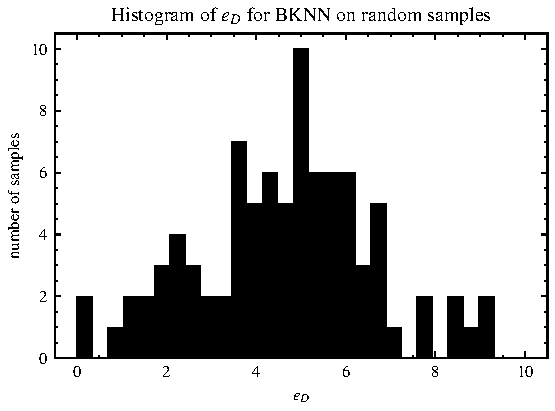
\includegraphics[width=\textwidth]{chapters/figures/result_histograms/result_histogram_random_sample_workload_dist_error_BKNN.pdf}
        \captionsetup{width=.9\linewidth}
        \caption{BKNN}
    \end{subfigure}%
    ~ 
    \begin{subfigure}[t]{0.5\textwidth}
        \centering
        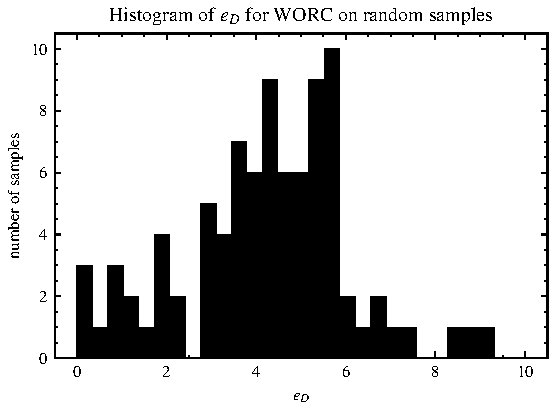
\includegraphics[width=\textwidth]{chapters/figures/result_histograms/result_histogram_random_sample_workload_dist_error_WORC.pdf}
        \captionsetup{width=.9\linewidth}
        \caption{WORC}
    \end{subfigure}
    \\[1ex]
    \centering
    \begin{subfigure}[t]{0.5\textwidth}
        \centering
        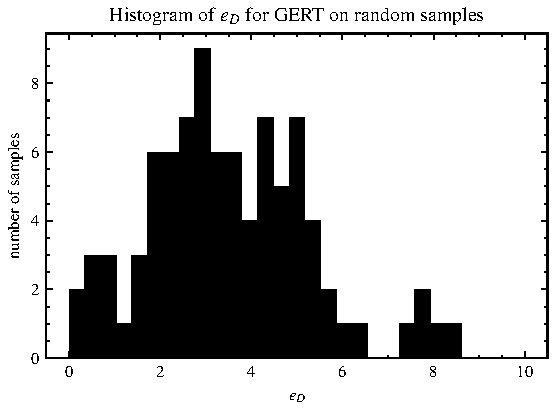
\includegraphics[width=\textwidth]{chapters/figures/result_histograms/result_histogram_random_sample_workload_dist_error_GERT.pdf}
        \captionsetup{width=.9\linewidth}
        \caption{GERT}
    \end{subfigure}%
    ~ 
    \begin{subfigure}[t]{0.5\textwidth}
        \centering
        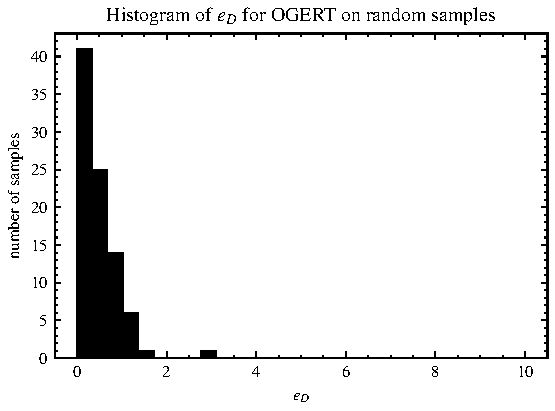
\includegraphics[width=\textwidth]{chapters/figures/result_histograms/result_histogram_random_sample_workload_dist_error_OGERT.pdf}
        \captionsetup{width=.9\linewidth}
        \caption{GORC}
    \end{subfigure}
    \caption{histogram of distribution error for the different models on the random splits dataset}
    \label{fig:result_random_sample_dist}
\end{figure}
%zone error histogram
\begin{figure}[ht]
    \centering
    \begin{subfigure}[t]{0.5\textwidth}
        \centering
        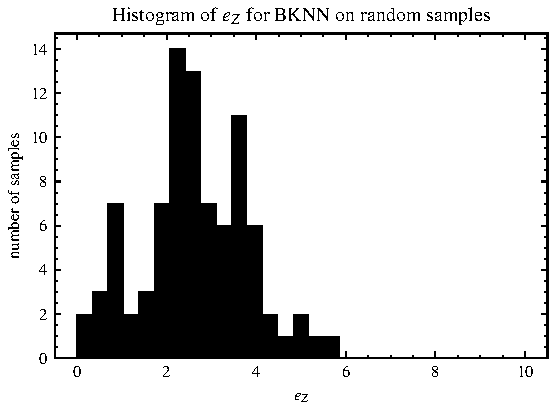
\includegraphics[width=\textwidth]{chapters/figures/result_histograms/result_histogram_random_sample_zone_sum_error_BKNN.pdf}
        \captionsetup{width=.9\linewidth}
        \caption{BKNN}
    \end{subfigure}%
    ~ 
    \begin{subfigure}[t]{0.5\textwidth}
        \centering
        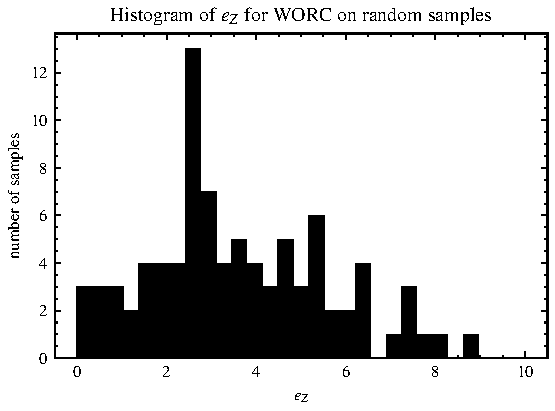
\includegraphics[width=\textwidth]{chapters/figures/result_histograms/result_histogram_random_sample_zone_sum_error_WORC.pdf}
        \captionsetup{width=.9\linewidth}
        \caption{WORC}
    \end{subfigure}
    \\[1ex]
    \centering
    \begin{subfigure}[t]{0.5\textwidth}
        \centering
        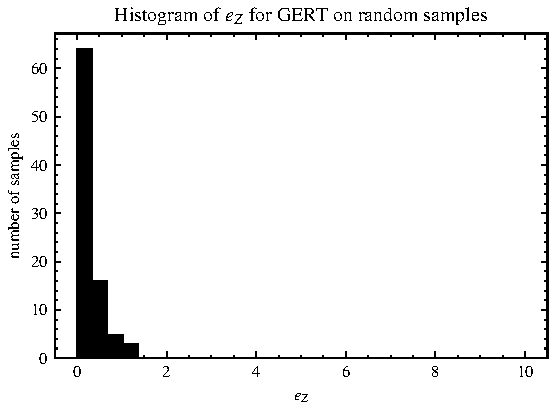
\includegraphics[width=\textwidth]{chapters/figures/result_histograms/result_histogram_random_sample_zone_sum_error_GERT.pdf}
        \captionsetup{width=.9\linewidth}
        \caption{GERT}
    \end{subfigure}%
    ~ 
    \begin{subfigure}[t]{0.5\textwidth}
        \centering
        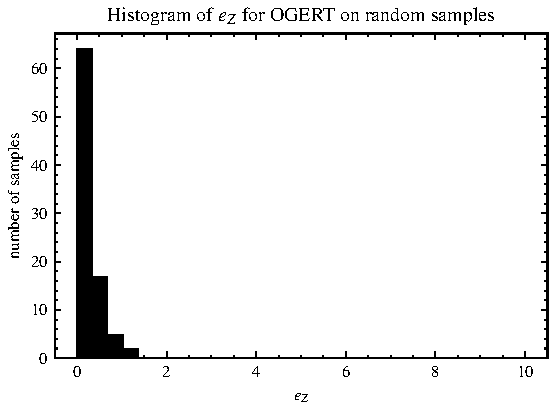
\includegraphics[width=\textwidth]{chapters/figures/result_histograms/result_histogram_random_sample_zone_sum_error_OGERT.pdf}
        \captionsetup{width=.9\linewidth}
        \caption{GORC}
    \end{subfigure}
    \caption{histogram of zone error for the different models on the random splits dataset}
    \label{fig:result_random_sample_dist}
\end{figure}

\subsection{last weeks}

%disitrbution error historgram
\begin{figure}[ht]
    \centering
    \begin{subfigure}[t]{0.5\textwidth}
        \centering
        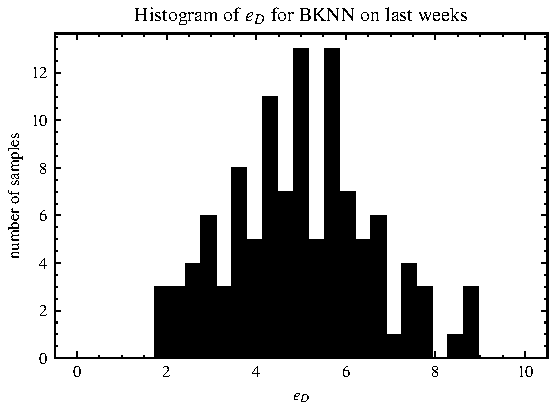
\includegraphics[width=\textwidth]{chapters/figures/result_histograms/result_histogram_last_weeks_workload_dist_error_BKNN.pdf}
        \captionsetup{width=.9\linewidth}
        \caption{BKNN}
    \end{subfigure}%
    ~ 
    \begin{subfigure}[t]{0.5\textwidth}
        \centering
        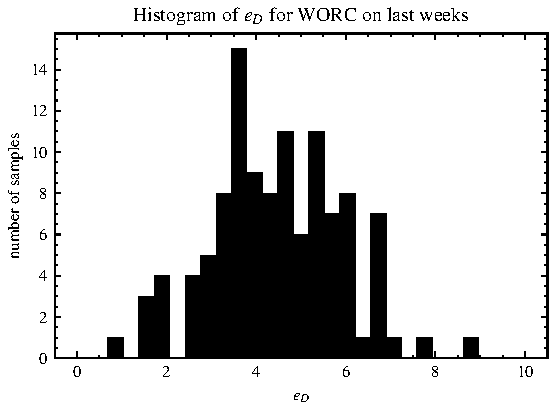
\includegraphics[width=\textwidth]{chapters/figures/result_histograms/result_histogram_last_weeks_workload_dist_error_WORC.pdf}
        \captionsetup{width=.9\linewidth}
        \caption{WORC}
    \end{subfigure}
    \\[1ex]
    \centering
    \begin{subfigure}[t]{0.5\textwidth}
        \centering
        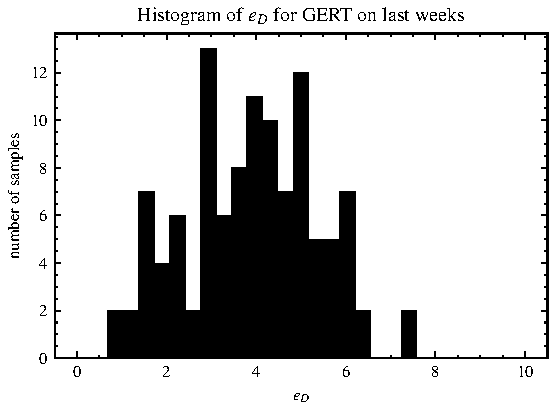
\includegraphics[width=\textwidth]{chapters/figures/result_histograms/result_histogram_last_weeks_workload_dist_error_GERT.pdf}
        \captionsetup{width=.9\linewidth}
        \caption{GERT}
    \end{subfigure}%
    ~ 
    \begin{subfigure}[t]{0.5\textwidth}
        \centering
        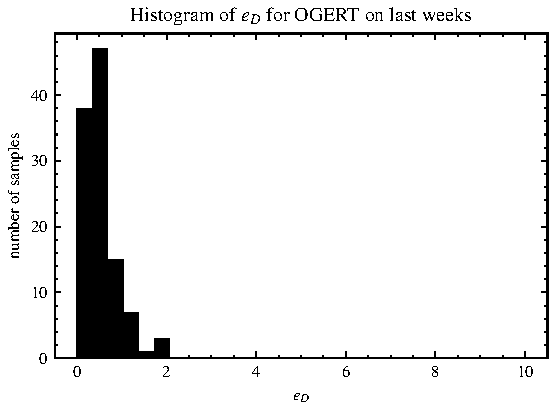
\includegraphics[width=\textwidth]{chapters/figures/result_histograms/result_histogram_last_weeks_workload_dist_error_OGERT.pdf}
        \captionsetup{width=.9\linewidth}
        \caption{GORC}
    \end{subfigure}
    \caption{histogram of distribution error for the different models on the random splits dataset}
    \label{fig:result_last_weeks_dist}
\end{figure}
%zone error histogram
\begin{figure}[ht]
    \centering
    \begin{subfigure}[t]{0.5\textwidth}
        \centering
        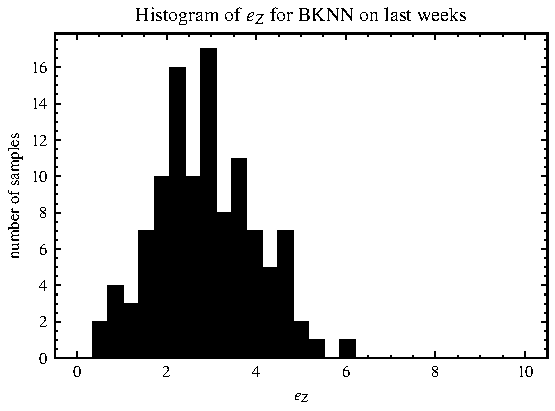
\includegraphics[width=\textwidth]{chapters/figures/result_histograms/result_histogram_last_weeks_zone_sum_error_BKNN.pdf}
        \captionsetup{width=.9\linewidth}
        \caption{BKNN}
    \end{subfigure}%
    ~ 
    \begin{subfigure}[t]{0.5\textwidth}
        \centering
        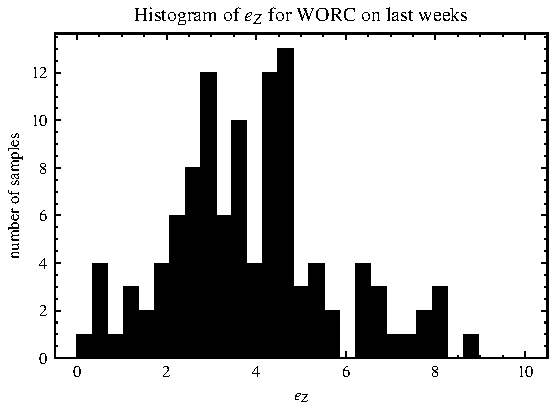
\includegraphics[width=\textwidth]{chapters/figures/result_histograms/result_histogram_last_weeks_zone_sum_error_WORC.pdf}
        \captionsetup{width=.9\linewidth}
        \caption{WORC}
    \end{subfigure}
    \\[1ex]
    \centering
    \begin{subfigure}[t]{0.5\textwidth}
        \centering
        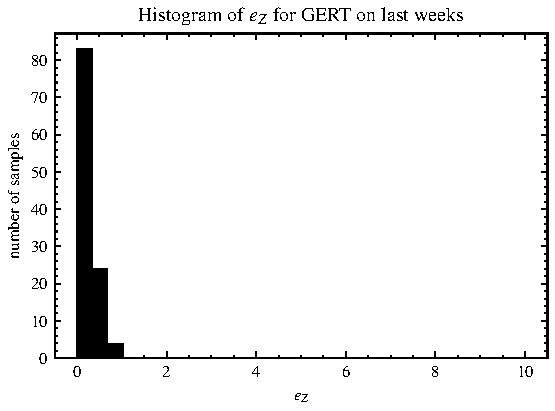
\includegraphics[width=\textwidth]{chapters/figures/result_histograms/result_histogram_last_weeks_zone_sum_error_GERT.pdf}
        \captionsetup{width=.9\linewidth}
        \caption{GERT}
    \end{subfigure}%
    ~ 
    \begin{subfigure}[t]{0.5\textwidth}
        \centering
        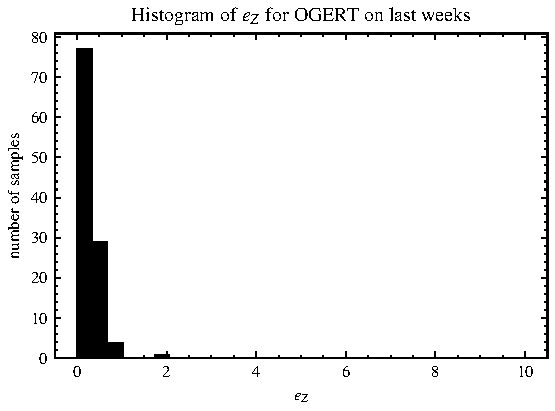
\includegraphics[width=\textwidth]{chapters/figures/result_histograms/result_histogram_last_weeks_zone_sum_error_OGERT.pdf}
        \captionsetup{width=.9\linewidth}
        \caption{GORC}
    \end{subfigure}
    \caption{histogram of zone error for the different models on the random splits dataset}
    \label{fig:result_last_weeks_dist}
\end{figure}

In \cref{fig:BKNN_pred,fig:GERT_pred} the total training load decided by the Basline KNN model and GERT respectively are plotted against the total training load decided by the coach for all training plans in test set \textit{random weeks}.
From the figures it is clear that the Baseline KNN model, even though it dose a descent job of mimicking the coach's total training load, is outperformed by the GERT model, which dose a near perfect job mimicking the coach's total training load.

\begin{figure}[ht]
    \centering
    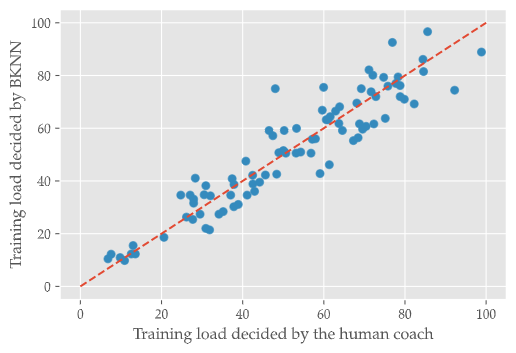
\includegraphics[width=0.8\textwidth]{chapters/figures/BKNN_predictions.png}
    \caption{Training load of weekly program set by the human coach versus that training program automatically generated by BKNN for all data points in the held-out test set. The dashed red line highlights the target function of perfect correspondence.}
    \label{fig:BKNN_pred}
\end{figure}

\begin{figure}[ht]
    \centering
    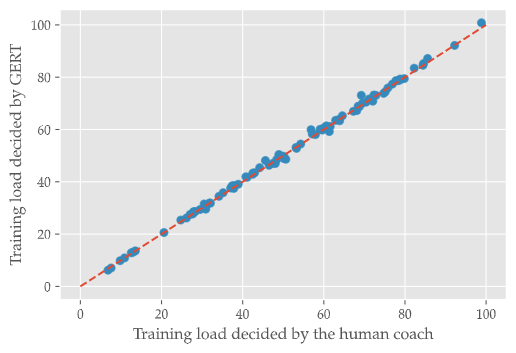
\includegraphics[width=0.8\textwidth]{chapters/figures/GERT_predictions.png}
    \caption{Training load of weekly program set by the human coach versus that training program automatically generated by GERT for all data points in the randomly sampled held-out test set. The dashed red line highlights the target function of perfect correspondence.}
    \label{fig:GERT_pred}
\end{figure}

When producing the results for \cref{fig:GERT_pred}, a typical workload, GERT took on average \SI{1.6}{\second} to generate a weekly plan on an ordinary workstation.\footnote{Intel\textregistered{} Core\texttrademark{} i7-3770 CPU @ 3.40GHz - 3 cores}

\todo{Follow up on the influence of the athlete parameters? Possibly with a feature importance analysis}

